\documentclass[conference]{IEEEtran}

% Packages
\usepackage[utf8]{inputenc}
\usepackage{amsmath,amssymb,amsfonts}
\usepackage{graphicx}
\usepackage{booktabs}
\usepackage[
  pdftitle={Reputation-Weighted Prediction Markets Under Wealth Heterogeneity and Heavy Tails},
  pdfauthor={estmcmxci.eth},
  pdfsubject={Reputation-weighted aggregation for prediction markets under wealth heterogeneity and heavy-tailed outcomes},
  pdfkeywords={prediction markets, reputation systems, forecast aggregation, heavy-tailed distributions, cultural markets, mechanism design},
  pdfcreator={LaTeX via pdflatex},
]{hyperref}
\usepackage{cite}
\usepackage{xcolor}
\usepackage{url}
\usepackage{microtype}              % Improved line breaking and spacing
\usepackage{balance}                % Balance last-page columns
\usepackage{enumitem}               % Compact lists

% Compact list spacing for itemize/enumerate
\setlist{nosep,leftmargin=*}
\setlist[enumerate]{label=\arabic*)}

% Tighter float spacing
\setlength{\textfloatsep}{8pt plus 2pt minus 2pt}
\setlength{\floatsep}{6pt plus 2pt minus 2pt}
\setlength{\intextsep}{6pt plus 2pt minus 2pt}
\setlength{\abovecaptionskip}{4pt}
\setlength{\belowcaptionskip}{2pt}

% Tighter equation spacing
\setlength{\abovedisplayskip}{6pt plus 2pt minus 2pt}
\setlength{\belowdisplayskip}{6pt plus 2pt minus 2pt}
\setlength{\abovedisplayshortskip}{3pt plus 1pt}
\setlength{\belowdisplayshortskip}{3pt plus 1pt}

\begin{document}

\title{Reputation-Weighted Prediction Markets Under Wealth Heterogeneity and Heavy Tails}

\author{
\IEEEauthorblockN{estmcmxci.eth}
\IEEEauthorblockA{Trece Research\\
New York City\\
m@oakgroup.co}
}

\date{February 14, 2026}

\maketitle

\begin{abstract}
Capital-weighted prediction markets assume that willingness to stake capital proxies for information quality. This assumption fails whenever outcomes are heavy-tailed, private information is heterogeneous, and wealth does not positively correlate with forecasting skill---conditions that co-occur in cultural breakout markets and other fat-tailed domains. We propose a reputation-weighted aggregation mechanism that learns agent quality endogenously from demonstrated forecasting accuracy and modulates each agent's influence as the product of reputation and stake ($w_i = r_i \cdot s_i$). Through Monte Carlo simulation under Pareto-distributed outcomes with heterogeneous private signals, we compare equal-weighted, capital-weighted, and reputation-weighted aggregation across three wealth--skill correlation regimes, parameter sweeps over tail heaviness and signal heterogeneity, and an inequality sensitivity sweep. Reputation-weighted aggregation improves over capital-weighted aggregation in every tested configuration ($p < 10^{-15}$ in main results), though the effect is modest ($+0.13\%$ to $+0.20\%$ in Brier score). Capital-weighting degrades forecasts by up to $5.27\%$ under extreme wealth concentration with anti-correlated wealth and skill. The reputation correction grows with inequality, noise gap, and tail heaviness, but the multiplicative architecture is the binding constraint: a ${\sim}10\%$ learned reputation differential cannot override a $40\times$ stake differential. The mechanism correctly identifies agent quality---reputation separation is invariant across all conditions---but lacks architectural authority to act proportionally on that knowledge. These findings motivate alternative weighting architectures that give demonstrated accuracy greater authority relative to raw capital. There is no tested configuration in which reputation-weighting degrades performance.
\end{abstract}

\begin{IEEEkeywords}
prediction markets, reputation systems, forecast aggregation, mechanism design, heavy-tailed distributions, cultural markets
\end{IEEEkeywords}

% ============================================================
\section{Introduction}
\label{sec:introduction}
% ============================================================

Prediction markets aggregate dispersed private information into probability estimates through capital-weighted price formation. A trader's influence on the market price is proportional to the capital they commit: larger bets move prices more~\cite{hanson2003,arrow2008}. This design embeds a tacit assumption---that willingness to stake capital is a reliable proxy for information quality. When it is, the market efficiently upweights informed participants. When it is not, the market systematically amplifies the beliefs of wealthy but uninformed traders at the expense of informed but capital-constrained ones.

This assumption fails whenever three conditions co-occur: outcomes are heavy-tailed, private information is heterogeneously distributed, and wealth does not positively correlate with forecasting skill. These conditions arise across economically important domains---venture capital deal selection, credit default prediction, pharmaceutical trial assessment, token launch markets---wherever payoffs are heavily skewed and the most informed participants are not the wealthiest. We study the problem in the context of cultural breakout markets, where all three conditions are structurally acute. These are prediction markets applied to whether a song, artist, film, or piece of content will achieve viral or commercial breakout. First, outcomes are heavy-tailed: most content fails, while a small number of items generate the vast majority of attention and revenue~\cite{clauset2009,salganik2006}. Second, private information is heterogeneous: some participants (early fans, tastemaker curators, niche community members) possess genuine forward-looking signal about which content will break out, while the majority do not~\cite{surowiecki2004}. Third, and critically, wealth does not correlate with forecasting skill in this domain. The participants with the best cultural signal are systematically not the wealthiest market participants. In the language of our model, this is Regime~B (anti-correlated wealth and skill)---not an edge case, but a structural feature of cultural prediction.

The practical consequence is visible in how cultural conviction is already valued informally. In fan communities, proof of early discovery---screenshots of following an artist before their breakout, timestamped playlist additions---circulates as social currency, with observable secondary-market transactions for these artifacts. Fig.~\ref{fig:depop} illustrates a representative example: a Depop listing offering a Spotify screenshot proving early listenership of the artist Nettspend---at the time showing 7,262 monthly listeners---for~\$5, with 38 prior sales from the same seller. The listing is not an anomaly; it is a market signal. It reveals latent demand for a system that converts conviction into verifiable taste: a record that is trustworthy, that compounds over time, and that can feed downstream decisions. But screenshots are forgeable, non-standardized, and non-composable. They prove presence, not prediction. The question is whether a formal mechanism can do better.

\begin{figure}[t]
    \centering
    
\includegraphics[width=\columnwidth]{nettspend.jpeg}
    \caption{Depop listing for a Spotify screenshot proving early listenership of the artist Nettspend (7,262 monthly listeners at time of capture), listed at~\$5. The seller has completed 38 transactions, indicating sustained demand for proof of early cultural conviction. Source: Depop, captured 2024.}
    \label{fig:depop}
\end{figure}

This paper proposes and evaluates a reputation-weighted aggregation mechanism for prediction markets operating under wealth heterogeneity and heavy-tailed outcomes. In our mechanism, each agent's influence on the aggregate forecast is proportional to the product of their stake and a learned reputation score: $w_i = r_i \cdot s_i$. The reputation score is updated after each round using an exponential moving average of the agent's forecasting accuracy, producing a slow-moving, stable summary of demonstrated skill. All agents begin with equal reputation; the mechanism must learn the quality differential from data. This multiplicative form preserves the skin-in-the-game incentive of capital-weighting while introducing a corrective factor that can amplify or attenuate each agent's influence based on their track record.

We evaluate this mechanism through Monte Carlo simulation, comparing three aggregation rules---equal-weighted, capital-weighted, and reputation-weighted---across three experimental campaigns:
\begin{enumerate}
    \item \textbf{Main results} (Section~\ref{sec:results-main}): Three wealth--skill correlation regimes (uncorrelated, anti-correlated, correlated) at default parameters, 30 seeds each.
    \item \textbf{Parameter sensitivity} (Section~\ref{sec:results-sweep}): Sweep over tail heaviness ($\alpha$) and noise gap ($\Delta\sigma$) for 18 configurations.
    \item \textbf{Inequality sensitivity} (Section~\ref{sec:results-inequality}): Sweep over stake dispersion ($\sigma_s$) from perfect equality to extreme concentration, 18 configurations.
\end{enumerate}
All three mechanisms observe the same private signals and the same realized outcomes on every round. Performance differences are therefore attributable solely to the weighting rule.

Our main findings are:
\begin{itemize}
    \item Reputation-weighted aggregation improves over capital-weighted aggregation in every tested configuration ($p < 10^{-15}$ in all main results), though the effect is modest in absolute magnitude ($+0.13\%$ to $+0.20\%$ in Brier score).
    \item Capital-weighting degrades forecast quality by up to $5.27\%$ relative to equal-weighting under extreme wealth concentration with anti-correlated wealth and skill.
    \item The reputation correction grows with wealth inequality, noise gap, and tail heaviness---it is largest precisely where the capital-weighting pathology is most severe.
    \item The multiplicative architecture is the binding constraint: the mechanism correctly identifies agent quality (reputation separation is invariant across all conditions) but a ${\sim}10\%$ reputation differential cannot override a $40\times$ stake differential. This motivates alternative weighting architectures explored in the Discussion.
    \item There is no tested configuration in which reputation-weighting degrades performance. It is safe to adopt even when capital already correlates with skill.
\end{itemize}

The paper is organized as follows. Section~\ref{sec:related} reviews related work on prediction markets, forecast aggregation, reputation systems, and heavy-tailed outcomes, and identifies the gaps this paper addresses. Section~\ref{sec:model} presents the model: the latent quality process, private signals, aggregation mechanisms, and reputation update rule. Section~\ref{sec:experiments} describes the experimental design, evaluation metrics, and statistical methods. Section~\ref{sec:results} reports results across the three campaigns. Section~\ref{sec:discussion} discusses interpretation of effect sizes, the architectural limitation, and implications for market design. Section~\ref{sec:limitations} addresses limitations and future work. Section~\ref{sec:conclusion} concludes.

% ============================================================
\section{Related Work}
\label{sec:related}
% ============================================================

\subsection{Prediction Markets and Capital-Weighted Aggregation}
\label{sec:related-markets}

Prediction markets aggregate dispersed private information into probability estimates through trading mechanisms. Wolfers and Zitzewitz (2004) provide the canonical survey, documenting that market-generated forecasts are typically well-calibrated and outperform moderately sophisticated benchmarks across domains including elections, economic indicators, and geopolitical events~\cite{wolfers2004}. The standard automated market maker is Hanson's Logarithmic Market Scoring Rule (LMSR), which combines the incentive-compatibility of proper scoring rules with the liquidity provision of a market maker, at a bounded worst-case cost controlled by the parameter~$b$~\cite{hanson2007}.

In all widely deployed prediction markets---whether order-book-based platforms like Polymarket or LMSR-based research platforms---a trader's influence on the market price is proportional to the capital they commit. Wolfers and Zitzewitz (2006) formalize this: under log utility, prediction market prices converge to the \emph{wealth-weighted} mean of traders' beliefs~\cite{wolfers2006}. This is the best-case interpretation. Manski (2006) shows that under alternative assumptions (risk-neutral agents with fixed budgets), prices may correspond to a quantile of the belief distribution rather than the mean, further undermining the prices-as-probabilities interpretation~\cite{manski2006}. The common thread is that capital-weighting is fundamentally \emph{wealth-weighting}, not information-weighting. When wealth correlates with forecasting skill, this distinction is immaterial. When it does not---as we argue is the case in cultural breakout markets---capital-weighting can actively degrade the aggregate forecast.

Snowberg and Wolfers (2010) document a specific manifestation of this problem: the favorite-longshot bias, in which low-probability events are systematically overpriced in betting markets~\cite{snowberg2010}. They attribute this to probability misperceptions rather than risk preferences, suggesting that calibration errors may be especially severe for the tail events that characterize cultural breakout prediction.

Despite this theoretical understanding, no prior work has experimentally tested how capital-weighted aggregation degrades under controlled variation in wealth inequality or in the correlation between wealth and forecasting skill. The Manski--Wolfers debate remains theoretical; our simulation provides the first direct test by manipulating both the degree of wealth concentration and the wealth--skill relationship across three distinct regimes.

\subsection{Performance-Weighted Forecast Aggregation}
\label{sec:related-aggregation}

An alternative to capital-weighting is to weight forecasters by demonstrated accuracy. Budescu and Chen (2015) develop methods to identify individual forecasters' contributions to crowd accuracy and construct optimally weighted aggregates, showing that even simple track-record-based weights substantially improve over equal-weight averaging~\cite{budescu2015}. Mellers et al.\ (2015) provide the empirical foundation for this approach by documenting ``superforecasters''---individuals who maintained top-2\% Brier scores across multiple seasons of the IARPA forecasting tournament---and showing that persistent, identifiable forecasting skill exists~\cite{mellers2015}. Atanasov et al.\ (2021) extend this line, demonstrating that forecaster accuracy is temporally stable and that simple performance-based weighting schemes capture most of the available improvement; more sophisticated methods (e.g., IRT-based) offer only marginal additional gains~\cite{atanasov2021}.

The most directly relevant empirical precedent is Atanasov et al.\ (2017), the first large-scale experimental comparison of prediction markets against prediction polls~\cite{atanasov2017}. They find that while market prices outperform simple mean polls, \emph{team prediction polls with differential weighting based on past performance outperform prediction markets}. This result---that performance-weighted aggregation can beat capital-weighted aggregation---is the central hypothesis our simulation formalizes and extends. However, Atanasov et al.\ do not control for wealth heterogeneity (all participants had comparable stakes in the experimental setting), nor do they test under heavy-tailed outcome distributions. Their events are geopolitical questions with relatively well-behaved base rates. Whether performance-weighting retains its advantage when wealth is explicitly heterogeneous and outcomes are power-law distributed remains untested.

In the expert judgment literature, Cooke's (1991) Classical Model derives performance-based weights from experts' accuracy on calibration ``seed'' variables with known true values~\cite{cooke1991}. Our reputation update rule can be viewed as an online, dynamic adaptation of the Classical Model: rather than calibrating on a fixed seed set, the mechanism continuously updates agent weights from the stream of resolved outcomes.

Additionally, no prior work has tested the \emph{safety} of adopting reputation-weighting: does it risk degrading performance when capital-weighting already works well (i.e., when wealth does correlate with skill)? This downside-risk question is critical for practical adoption.

\subsection{Proper Scoring Rules}
\label{sec:related-scoring}

Our evaluation relies on two strictly proper scoring rules. The Brier score, introduced by Brier (1950), measures the mean squared error between probabilistic forecasts and binary outcomes~\cite{brier1950}. The logarithmic scoring rule, which also underpins the LMSR, penalizes confident incorrect predictions more severely. Gneiting and Raftery (2007) provide the modern characterization: a scoring rule is strictly proper if and only if it can be expressed in terms of a convex entropy function and its associated Bregman divergence~\cite{gneiting2007}. We report both Brier and log loss to ensure our results are not artifacts of a particular scoring rule's sensitivity profile.

Our reputation update rule uses an exponential credit function, $\exp(-k(p_i - Y)^2)$, which is closely related to the Brier score. The use of proper scoring rules for reputation computation ensures that agents maximize their expected reputation by reporting truthfully---an incentive-compatibility property inherited from the scoring rule literature.

\subsection{Heavy-Tailed Distributions and Cultural Markets}
\label{sec:related-tails}

Cultural consumption follows heavy-tailed distributions. Elberse (2013) documents empirically that entertainment industry outcomes are extremely right-skewed: a small number of products generate the vast majority of revenue, while most fail~\cite{elberse2013}. Shapiro (2023) explains the mechanism: as content supply grows, consumers rely more heavily on social signals and recommendation algorithms, which concentrate attention and produce power-law-distributed breakout events~\cite{shapiro2023}. This structural feature---most items fail, a few explode---is the empirical basis for the Pareto-distributed latent quality in our simulation.

Taleb (2020) characterizes the statistical consequences of fat tails: standard estimators (mean, variance) converge slowly or not at all, the Law of Large Numbers requires far more samples, and calibration of tail parameters is inherently fragile~\cite{taleb2020}. For prediction market design, this means that scoring and reputation systems must be evaluated under heavy-tailed outcome distributions, not just well-behaved ones. Yet the prediction market literature has largely evaluated mechanism performance under bounded or thin-tailed outcomes. Whether reputation-weighted aggregation maintains its advantage under the heavy tails characteristic of cultural markets---and whether the advantage scales with tail heaviness---has not been tested.

\subsection{Summary of Gaps and Contribution}
\label{sec:related-gaps}

To summarize, the existing literature establishes that (a)~capital-weighted markets are wealth-weighted by construction~\cite{wolfers2006,manski2006}, (b)~performance-based weighting can improve forecast aggregation~\cite{budescu2015,mellers2015,atanasov2017}, and (c)~cultural outcomes are heavy-tailed~\cite{elberse2013,shapiro2023}. However, no prior work has experimentally tested how capital-weighted aggregation degrades under controlled variation in wealth inequality, wealth--skill correlation, and tail heaviness---nor whether reputation-weighted aggregation corrects this degradation across all three dimensions simultaneously. Crucially, no prior work has tested whether reputation-weighting is safe to adopt even when capital already correlates with skill, a necessary condition for practical deployment. This paper provides that test.

% ============================================================
\section{Model}
\label{sec:model}
% ============================================================

\subsection{Setup and Notation}
\label{sec:model-setup}

We consider a sequential prediction setting with $N$ agents indexed $i = 1, \dots, N$ evaluating $J$ content items (e.g., songs, videos, posts) in succession. Each agent~$i$ is characterized by a private signal precision $\sigma_i > 0$ (lower is better) and a stake $s_i \geq 0$ representing the capital they commit to the market. Agents are partitioned into two types: a fraction~$\phi$ are \emph{good} agents with signal noise $\sigma_{\text{good}}$, and the remaining $1 - \phi$ are \emph{bad} agents with signal noise $\sigma_{\text{bad}} > \sigma_{\text{good}}$. The difference $\Delta\sigma = \sigma_{\text{bad}} - \sigma_{\text{good}}$ is the \emph{noise gap}, which parameterizes the degree of skill heterogeneity in the population.

This binary partition is a simplification of continuous skill distributions, chosen because it isolates the core question: can the mechanism learn to upweight the informed minority even when that minority holds less capital? The 80/20 split ($\phi = 0.2$) models the empirically common situation where the majority of market participants are noise traders or casual bettors, while a small minority possesses genuine predictive skill~\cite{mellers2015,atanasov2017}.

\subsection{Latent Quality and Breakout Probability}
\label{sec:model-quality}

For each item~$j$, a latent quality $q_j$ is drawn from a shifted Pareto distribution:
\begin{equation}
    q_j \sim \text{Pareto}(\alpha) + 1, \quad f(q) = \alpha \, q^{-(\alpha+1)}, \quad q \geq 1
\end{equation}

The Pareto distribution is chosen because cultural breakout events---streaming counts, viral reach, box office returns---empirically follow power-law distributions~\cite{elberse2013,shapiro2023}. The shape parameter $\alpha > 1$ controls tail heaviness: smaller $\alpha$ produces heavier tails with more extreme outliers. We test $\alpha \in \{1.3, 1.7, 2.5\}$, spanning from very heavy ($\alpha = 1.3$, finite mean but infinite variance) to moderately heavy ($\alpha = 2.5$) tails.

The latent quality is mapped to a true breakout probability via a sigmoid transform:
\begin{equation}
    \theta_j = \sigma(\beta \log q_j + b)
\end{equation}
where $\sigma(x) = 1/(1 + e^{-x})$ is the logistic sigmoid and $\beta = 1$ is a scaling constant. The logarithmic compression of $q_j$ is essential: without it, the Pareto's heavy tail would produce extreme values of the sigmoid argument, collapsing most breakout probabilities to 0 or~1 and eliminating the interesting forecasting problem in the interior of the probability simplex.

The bias~$b$ is calibrated so that $\mathbb{E}[\theta_j] \approx 0.10$---i.e., approximately 10\% of items break out. This base rate reflects the empirical reality of cultural markets, where the vast majority of content fails to achieve viral or commercial breakout~\cite{elberse2013}. Calibration is performed via Brent's root-finding method on a sample of 200,000 Pareto draws, and $b$~is recalibrated for each value of~$\alpha$ to ensure a constant base rate across tail-heaviness comparisons.

\subsection{Private Signals and Beliefs}
\label{sec:model-signals}

Each agent~$i$ observes a private signal about item~$j$ in log-odds space:
\begin{equation}
    x_{i,j} = \text{logit}(\theta_j) + \epsilon_{i,j}, \quad \epsilon_{i,j} \sim \mathcal{N}(0, \sigma_i^2)
\end{equation}
where $\text{logit}(p) = \log(p/(1-p))$. Working in log-odds space ensures that additive Gaussian noise is symmetric around the true value and that the transform back to probability space via the sigmoid naturally constrains beliefs to $[0, 1]$.

Agent~$i$'s belief is then:
\begin{equation}
    p_{i,j} = \sigma(x_{i,j})
\end{equation}%
Good agents ($\sigma_i = 0.6$) produce beliefs tightly clustered around~$\theta_j$; bad agents ($\sigma_i = 1.6$) produce beliefs that are substantially more dispersed. To give concrete intuition: for a true $\theta = 0.10$, a good agent's beliefs are typically in the range $[0.04, 0.22]$, while a bad agent's beliefs range from roughly $[0.01, 0.60]$. The bad agent's signal is wide enough to be nearly uninformative on any individual round, though it is still unbiased in expectation.

\subsection{Aggregation Mechanisms}
\label{sec:model-aggregation}

We compare three aggregation rules that map the vector of individual beliefs $(p_{1,j}, \dots, p_{N,j})$ to a single consensus probability for each item~$j$.

\textbf{Equal-weighted (baseline).} The unweighted crowd average:
\begin{equation}
    \bar{p}_j = \frac{1}{N} \sum_{i=1}^{N} p_{i,j}
\end{equation}
This ignores both capital and track record. It serves as the reference against which capital-weighting is measured.

\textbf{Capital-weighted.} Each agent's belief is weighted by their stake~$s_i$:
\begin{equation}
    p_j^C = \frac{\sum_{i=1}^{N} s_i \, p_{i,j}}{\sum_{i=1}^{N} s_i}
\end{equation}
This is the mechanism implicit in all existing capital-weighted prediction markets. In an order-book market like Polymarket, a trader's influence on the market price is proportional to their order size; in an LMSR-based market, it is proportional to the number of shares purchased. The capital-weighted average is a simplified stand-in that captures the core property: \emph{influence is proportional to stake, with no use of past accuracy}~\cite{wolfers2006,manski2006}. This simplification removes sequential trading dynamics and price impact but preserves the fundamental aggregation principle that our experiment targets.

\textbf{Reputation-weighted (proposed).} Each agent's belief is weighted by the product of their stake and a learned reputation score~$r_i$:
\begin{equation}
    p_j^R = \frac{\sum_{i=1}^{N} r_i \, s_i \, p_{i,j}}{\sum_{i=1}^{N} r_i \, s_i}
\end{equation}
The multiplicative form $r_i \cdot s_i$ preserves the skin-in-the-game incentive of capital-weighting while introducing a corrective factor that can amplify or attenuate each agent's influence based on demonstrated forecasting quality.

All three mechanisms observe the \emph{same} individual beliefs $p_{i,j}$ on every round. The only difference is the weighting scheme. Any performance difference is therefore attributable solely to the aggregation rule.

\subsection{Scoring and Reputation Update}
\label{sec:model-reputation}

After each round, the binary outcome $Y_j \sim \text{Bernoulli}(\theta_j)$ is observed and used to score the aggregate forecasts and update reputations.

\textbf{Scoring.} We evaluate each mechanism using two strictly proper scoring rules:
\begin{itemize}
    \item \emph{Brier score:} $\text{BS}_j = (\hat{p}_j - Y_j)^2$
    \item \emph{Log loss:} $\text{LL}_j = -[Y_j \log \hat{p}_j + (1 - Y_j) \log(1 - \hat{p}_j)]$
\end{itemize}
where $\hat{p}_j$ is the mechanism's aggregate forecast, clipped to $[10^{-6}, 1 - 10^{-6}]$ to prevent numerical overflow in the log loss.

\textbf{Reputation update.} After observing $Y_j$, each agent's reputation is updated via an exponential moving average (EMA) with exponential credit:
\begin{equation}
    r_i \leftarrow (1 - \lambda) \, r_i + \lambda \exp\!\big(-k (p_{i,j} - Y_j)^2\big)
\end{equation}%
All agents are initialized with $r_i = 1$. The update has three components:
\begin{enumerate}
    \item \emph{Exponential credit:} $\exp(-k(p_{i,j} - Y_j)^2)$ produces a score in $(0, 1]$. If agent~$i$'s prediction was close to the outcome, the credit is near~1; if far, it decays exponentially toward~0. The parameter $k = 5$ controls the sharpness of this decay.
    \item \emph{EMA smoothing:} The parameter $\lambda = 0.05$ determines how quickly reputation responds to new evidence. With $\lambda = 0.05$, approximately 95\% of the weight is on the agent's history, making reputation a slow-moving, stable summary of past performance. This prevents a single lucky or unlucky round from dominating the reputation signal.
    \item \emph{Initialization at unity:} All agents start with equal reputation, meaning the reputation-weighted mechanism is identical to capital-weighted on round~1. The mechanism must \emph{learn} the quality differential from data; it has no prior information about which agents are good.
\end{enumerate}

The exponential credit function is closely related to the Brier score---both measure squared error between prediction and outcome. This connection to proper scoring rules ensures that, in expectation, agents maximize their accumulated reputation by reporting truthfully.

\textbf{Order of operations.} The reputation used to weight round~$j$'s forecast is learned from rounds~$1$ through $j{-}1$. Reputation is updated \emph{after} scoring, never benefiting from hindsight on the current round. This is the standard online learning setup.

\subsection{Heterogeneous Stakes and Wealth--Skill Regimes}
\label{sec:model-stakes}

Stakes are drawn from a log-normal distribution and normalized to unit mean:
\begin{equation}
    \tilde{s}_i \sim \text{LogNormal}(0, \sigma_s^2), \quad s_i = \tilde{s}_i \, / \, \overline{\tilde{s}}
\end{equation}
The log-normal distribution is the standard model for wealth and income distributions---right-skewed, always positive, and parameterized by a single dispersion parameter~$\sigma_s$. Normalization to mean~1 ensures that the total capital in the market is constant across inequality levels; only the \emph{distribution} of capital changes.

At $\sigma_s = 0$, all agents have stake $s_i = 1$ and the capital-weighted mechanism is mathematically identical to equal-weighted. As $\sigma_s$ increases, wealth concentration grows: at $\sigma_s = 1.0$, the Gini coefficient is approximately 0.47 and the top 20\% of agents hold roughly 2--3$\times$ the capital of the bottom 80\%. At $\sigma_s = 2.0$, Gini reaches 0.73, comparable to crypto wealth distributions, and a handful of agents dominate the capital-weighted forecast.

We define three \emph{wealth--skill correlation regimes} that control how stakes are assigned to agent types:

\textbf{Regime A (Uncorrelated).} Stakes are assigned to agents uniformly at random, independently of their signal precision. Wealth carries no information about skill.

\textbf{Regime B (Anti-correlated).} Agents are processed in descending order of stake. Each agent is assigned to the ``bad'' (high-noise) pool with probability~0.8 and to the ``good'' (low-noise) pool with probability~0.2, subject to the constraint that pool sizes match the $\phi / (1-\phi)$ split. This produces a population where high-stake agents are predominantly noisy forecasters---the adversarial case for capital-weighting.

\textbf{Regime C (Correlated).} The mirror of Regime~B: high-stake agents are assigned to the good pool with probability~0.8. This is the best case for capital-weighting, where wealth proxies for skill.

The probabilistic (80/20) assignment rather than deterministic sorting reflects the reality that wealth--skill correlations are never perfect. Even in Regime~B, some whales happen to be skilled; even in Regime~C, some small players are good forecasters. This softening prevents pathological edge cases and makes the regimes more empirically realistic.

Stakes are regenerated independently for each random seed, meaning that multi-seed results average over both randomness in outcomes \emph{and} randomness in the wealth distribution.

% ============================================================
\section{Experimental Design}
\label{sec:experiments}
% ============================================================

\subsection{Simulation Protocol}
\label{sec:experiments-protocol}

Each experimental run is a single invocation of the model pipeline (Sections~\ref{sec:model-quality} through~\ref{sec:model-reputation}) for $J$~rounds with a fixed random seed. A single pseudorandom number generator (NumPy \texttt{default\_rng}) initialized with the seed produces all stochastic quantities---Pareto draws, agent noise, Bernoulli outcomes, and stake draws---in a deterministic sequence.

This design ensures that for a given seed, all three aggregation mechanisms observe the \emph{same} latent qualities, the \emph{same} private signals, and the \emph{same} realized outcomes. The only variable is the weighting rule. Performance differences across mechanisms are therefore attributable solely to the aggregation scheme, not to sampling variation. This paired structure is critical for statistical power: rather than asking whether reputation outperforms capital \emph{on average across different worlds}, we ask whether it outperforms \emph{in the same world}---a far more powerful test that dramatically reduces variance.

\subsection{Evaluation Metrics}
\label{sec:experiments-metrics}

For each mechanism $m \in \{E, C, R\}$ and seed~$s$, we compute the mean Brier score $\overline{\text{BS}}_m^{(s)} = J^{-1} \sum_j \text{BS}_{m,j}^{(s)}$ and mean log loss $\overline{\text{LL}}_m^{(s)} = J^{-1} \sum_j \text{LL}_{m,j}^{(s)}$ across all $J$~rounds.

The primary outcome variable is the relative improvement of reputation-weighted over capital-weighted aggregation:
\begin{equation}
    \Delta_{R \text{ vs } C}^{(s)} = \frac{\overline{S}_C^{(s)} - \overline{S}_R^{(s)}}{\overline{S}_C^{(s)}} \times 100\%
\end{equation}
where $S$ is either Brier score or log loss. Positive values indicate that reputation outperforms capital. We report this for both scoring rules to guard against artifacts of any single metric's sensitivity profile.

As a secondary outcome, we report the \emph{capital distortion}:
\begin{equation}
    \Delta_{C \text{ vs } E}^{(s)} = \frac{\overline{S}_E^{(s)} - \overline{S}_C^{(s)}}{\overline{S}_E^{(s)}} \times 100\%
\end{equation}
Positive values indicate that capital-weighting improves over equal-weighting; negative values indicate that capital-weighting \emph{degrades} the forecast. This metric isolates the effect of wealth heterogeneity on the capital-weighted mechanism, independent of the reputation correction.

We also track \emph{reputation separation}---the ratio of mean final reputation among good agents to mean final reputation among bad agents---as a measure of the mechanism's ability to identify agent quality endogenously.

\subsection{Statistical Methods}
\label{sec:experiments-stats}

For each experimental configuration (regime, parameter setting), we run $n$ independent seeds and obtain $n$ paired improvement values $\{\Delta^{(1)}, \dots, \Delta^{(n)}\}$.

\textbf{Confidence intervals.} We construct 95\% confidence intervals for the mean improvement via the nonparametric bootstrap (10,000 resamples with replacement). The bootstrap avoids distributional assumptions, which is appropriate given that the improvement values are ratios of correlated random variables.

\textbf{Hypothesis testing.} We test $H_0\!: \mathbb{E}[\Delta] = 0$ using a paired one-sample $t$-test on the $n$ per-seed improvement values. The paired design---same seed, different mechanism---ensures that the test captures the mechanism effect rather than cross-seed variance. We report $p$-values with significance levels $*$~($p < 0.05$), $**$~($p < 0.01$), $***$~($p < 0.001$).

\subsection{Parameter Settings}
\label{sec:experiments-params}

Table~\ref{tab:params} summarizes the default parameter values and swept ranges.

\begin{table}[t]
\centering
\caption{Default Simulation Parameters}
\label{tab:params}
\begin{tabular}{@{}llll@{}}
\toprule
\textbf{Parameter} & \textbf{Symbol} & \textbf{Default} & \textbf{Swept} \\
\midrule
Agents & $N$ & 50 & --- \\
Rounds & $J$ & 5{,}000 & 2{,}000 \\
Pareto tail & $\alpha$ & 1.7 & \{1.3, 1.7, 2.5\} \\
Base rate & $\mathbb{E}[\theta]$ & 0.10 & --- \\
Good fraction & $\phi$ & 0.20 & --- \\
Good noise & $\sigma_{\text{good}}$ & 0.6 & --- \\
Bad noise & $\sigma_{\text{bad}}$ & 1.6 & \{1.1, 1.6, 2.1\} \\
Stake dispersion & $\sigma_s$ & 1.0 & 0.0--2.0 \\
Rep.\ learning rate & $\lambda$ & 0.05 & --- \\
Rep.\ sharpness & $k$ & 5.0 & --- \\
Rep.\ initialization & $r_0$ & 1.0 & --- \\
\bottomrule
\end{tabular}
\end{table}

\subsection{Experimental Campaigns}
\label{sec:experiments-campaigns}

We conduct three experimental campaigns, each targeting a different dimension of the research question.

\textbf{Campaign 1: Main results} (Section~\ref{sec:results-main}). All three regimes (A, B, C) at default parameters. $J = 5{,}000$ rounds, $n = 30$ seeds per regime. This establishes the core finding: does reputation outperform capital, and does the answer depend on the wealth--skill correlation?

\textbf{Campaign 2: Parameter sensitivity} (Section~\ref{sec:results-sweep}). Sweep over $\alpha \in \{1.3, 1.7, 2.5\}$ and noise gap $\Delta\sigma \in \{0.5, 1.0, 1.5\}$ for Regimes~A and~B. $J = 2{,}000$, $n = 10$ seeds per cell. This tests robustness across tail heaviness and signal heterogeneity: $3 \times 3 \times 2 = 18$ configurations.

\textbf{Campaign 3: Inequality sensitivity} (Section~\ref{sec:results-inequality}). Sweep $\sigma_s \in \{0.0, 0.25, 0.50, \dots, 2.0\}$ for Regimes~A and~B at default signal parameters. $J = 5{,}000$, $n = 20$ seeds per cell. This tests how wealth concentration affects both the capital distortion and the reputation correction: $9 \times 2 = 18$ configurations. The $\sigma_s = 0$ anchor provides a built-in sanity check: with equal stakes, capital-weighted must equal equal-weighted exactly.

In total, the three campaigns comprise $3 \times 30 + 18 \times 10 + 18 \times 20 = 630$ simulation runs, each of $J = 2{,}000$--$5{,}000$ rounds.

% ============================================================
\section{Results}
\label{sec:results}
% ============================================================

\subsection{Main Results: Three Wealth--Skill Regimes}
\label{sec:results-main}

Table~\ref{tab:main-results} presents the core results across all three wealth--skill correlation regimes at default parameters ($\alpha = 1.7$, $\sigma_{\text{good}} = 0.6$, $\sigma_{\text{bad}} = 1.6$, $\sigma_s = 1.0$, $J = 5{,}000$, $n = 30$ seeds).

\begin{table*}[t]
\centering
\caption{Reputation vs.\ Capital Improvement Across Wealth--Skill Regimes}
\label{tab:main-results}
\begin{tabular}{@{}llccccc@{}}
\toprule
\textbf{Regime} & \textbf{Metric} & \textbf{R vs C (\%)} & \textbf{95\% CI} & $\boldsymbol{p}$\textbf{-value} & \textbf{C vs E (\%)} & \textbf{Rep Sep} \\
\midrule
A: Uncorrelated     & Brier   & $+0.155$ & $[+0.143,\, +0.166]$ & $1.2 \times 10^{-21}$ *** & $-0.834$ & $1.105\times$ \\
A: Uncorrelated     & LogLoss & $+0.152$ & $[+0.141,\, +0.162]$ & $4.1 \times 10^{-22}$ *** & $-0.586$ & $1.105\times$ \\
B: Anti-correlated  & Brier   & $+0.138$ & $[+0.123,\, +0.156]$ & $4.8 \times 10^{-16}$ *** & $-1.213$ & $1.105\times$ \\
B: Anti-correlated  & LogLoss & $+0.132$ & $[+0.117,\, +0.148]$ & $2.4 \times 10^{-16}$ *** & $-0.925$ & $1.105\times$ \\
C: Correlated       & Brier   & $+0.145$ & $[+0.134,\, +0.156]$ & $3.5 \times 10^{-21}$ *** & $+1.881$ & $1.105\times$ \\
C: Correlated       & LogLoss & $+0.170$ & $[+0.161,\, +0.180]$ & $3.5 \times 10^{-25}$ *** & $+2.191$ & $1.105\times$ \\
\bottomrule
\end{tabular}
\vspace{2pt}

{\small R vs C: positive = reputation outperforms capital. C vs E: positive = capital improves over equal-weighting; negative = capital degrades.}
\end{table*}

\begin{figure}[t]
    \centering
    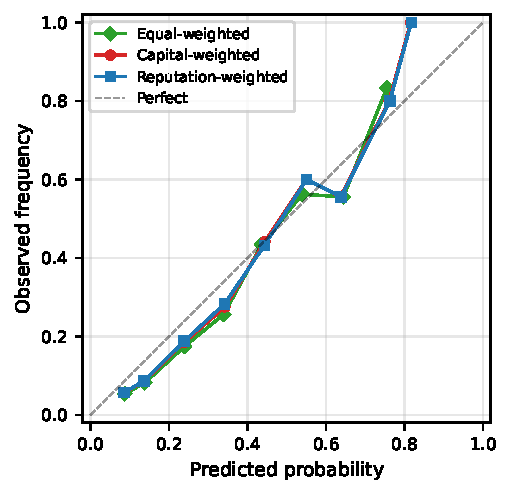
\includegraphics[width=\columnwidth]{fig_calibration.pdf}
    \caption{Calibration plot comparing all three aggregation mechanisms (Regime~B, seed~42, $J = 5{,}000$). Each point shows the observed breakout frequency within a predicted-probability bin. All three mechanisms are well-calibrated; the reputation-weighted curve (blue squares) tracks the diagonal most closely.}
    \label{fig:calibration}
\end{figure}

\smallskip\noindent\textbf{Finding 1: Reputation-weighted aggregation improves over capital-weighted aggregation in all three regimes, though the effect is modest in absolute magnitude.} The R-vs-C improvement is positive and highly statistically significant ($p < 10^{-15}$) across all six tests (3 regimes $\times$ 2 metrics), with 95\% confidence intervals entirely above zero. The improvement ranges from $+0.14\%$ to $+0.16\%$ in Brier score ($+0.13\%$ to $+0.17\%$ across both metrics)---a consistent but small correction. This result holds regardless of whether wealth correlates with skill, is independent of it, or inversely correlates with it.

\smallskip\noindent\textbf{Finding 2: Capital-weighting degrades forecast quality when wealth does not positively correlate with skill.} The C-vs-E column reveals the directional effect of capital-weighting relative to equal-weighting. In Regime~A (uncorrelated), capital-weighting reduces Brier accuracy by $0.83\%$---introducing noise by randomly overweighting some agents and underweighting others. In Regime~B (anti-correlated), the degradation is more severe at $1.21\%$---capital-weighting systematically amplifies the influence of noisy agents. Only in Regime~C (correlated), where whales are predominantly skilled, does capital-weighting help ($+1.88\%$ Brier). Notably, the capital distortion in Regimes~A and~B is 5--9$\times$ larger in magnitude than the reputation correction, foreshadowing a key limitation explored in Section~\ref{sec:results-inequality}.

\smallskip\noindent\textbf{Finding 3: Reputation-weighting never underperforms capital-weighting, but provides only a partial correction.} Regime~C is the best-case scenario for capital-weighting---wealth already proxies for skill, and capital-weighted aggregation outperforms equal-weighted by nearly 2\%. Even here, reputation-weighted aggregation further improves over capital-weighted by $+0.145\%$ (Brier) and $+0.170\%$ (LogLoss), both with $p < 10^{-20}$. There is no tested configuration in which reputation-weighting degrades performance. However, the magnitude of the reputation correction ($+0.13$--$0.17\%$) is an order of magnitude smaller than the capital distortion it corrects in Regimes~A and~B ($-0.83\%$ to $-1.21\%$). This asymmetry is structural, not incidental: because the reputation-weighted forecast is $p^R = \sum r_i s_i p_i / \sum r_i s_i$, each agent's influence is \emph{bounded below by their stake}. Reputation can modulate stake---scaling it up or down by a small factor---but cannot override it. A consistently accurate minnow accumulates high reputation, yet their effective weight $r_i \cdot s_i$ remains small when $s_i$ is small. Reputation-weighting is safe to adopt but is not a full remedy for capital-weighting pathologies under this multiplicative architecture.

\smallskip\noindent\textbf{Finding 4: Reputation separation is invariant to the wealth structure.} The mechanism achieves a reputation separation ratio of $1.105\times$ in the main results (good agents accumulate ${\sim}10\%$ higher reputation than bad agents) identically across all three regimes. This confirms that the reputation learning rule identifies agent quality from forecasting accuracy alone, independent of agents' stake levels. Whether a good agent is a whale (Regime~C) or a minnow (Regime~B), they still make better predictions and accumulate proportionally more reputation. However, the modest separation ratio of $1.105\times$ also explains the modest effect sizes: a ${\sim}10\%$ reputation differential can only partially offset stake differentials between agents.

\subsection{Parameter Sensitivity}
\label{sec:results-sweep}

To assess robustness beyond the default parameter setting, we sweep over $\alpha \in \{1.3, 1.7, 2.5\}$ (tail heaviness) and noise gap $\Delta\sigma \in \{0.5, 1.0, 1.5\}$ (signal heterogeneity) for Regimes~A and~B ($J = 2{,}000$, $n = 10$ seeds per cell).

\smallskip\noindent\textbf{Finding 5: The reputation advantage scales monotonically with the noise gap.} As the difference between good and bad agent precision increases from $\Delta\sigma = 0.5$ to $\Delta\sigma = 1.5$, the R-vs-C Brier improvement grows from approximately $+0.01\%$ (often non-significant at $\Delta\sigma = 0.5$) to $+0.50\%$ ($p < 10^{-5}$ at $\Delta\sigma = 1.5$). This scaling is smooth and monotonic across all tested $\alpha$ values and both regimes. The interpretation is straightforward: when there is more skill heterogeneity to exploit, the reputation mechanism extracts more value from it.

\smallskip\noindent\textbf{Finding 6: The reputation advantage scales with tail heaviness.} {\looseness=-1 At a fixed noise gap, higher $\alpha$ (lighter tails) produces larger R-vs-C improvements. This may appear counterintuitive---heavier tails make forecasting harder, so one might expect more room for reputation to help. However, lighter tails produce a cleaner signal-to-noise ratio in the reputation update: breakout probabilities are less extreme, so the squared error $(p_i - Y)^2$ is more informative about agent quality. The mechanism learns faster and separates agents more cleanly under lighter tails.\par}

\smallskip\noindent\textbf{Finding 7: The mechanism never hurts.} Across all 36 cells of the parameter sweep (2 regimes $\times$ 3 $\alpha$ $\times$ 3 noise gaps $\times$ 2 metrics), the mean R-vs-C improvement is non-negative in every case. At the low end ($\alpha = 1.3$, $\Delta\sigma = 0.5$), some results are not statistically significant, reflecting limited statistical power with 10 seeds and a genuinely small effect. But the point estimate is always positive or near zero---there is no cell where reputation-weighting is harmful.

\subsection{Inequality Sensitivity}
\label{sec:results-inequality}

The main results (Section~\ref{sec:results-main}) use $\sigma_s = 1.0$, corresponding to moderate wealth inequality (Gini $\approx 0.47$). To test how the degree of wealth concentration affects both the capital-weighting pathology and the reputation correction, we sweep $\sigma_s$ from 0.0 (perfect equality) to 2.0 (extreme concentration, Gini $\approx 0.73$) for Regimes~A and~B ($J = 5{,}000$, $n = 20$ seeds per cell). This sweep reveals the central limitation of multiplicative reputation-weighting: as wealth concentration increases, noisy whales increasingly dominate the aggregate forecast, and a small multiplicative adjustment to their weight cannot undo the distortion their stake imposes.

\smallskip\noindent\textbf{Finding 8: At $\sigma_s = 0$, capital-weighted is identical to equal-weighted (sanity check).} When all agents have stake $s_i = 1$, the capital-weighted and equal-weighted forecasts are mathematically identical. The measured C-vs-E delta is ${<}\,10^{-15}\%$ (floating-point zero), and results are identical across Regimes~A and~B---confirming that the regime assignment is irrelevant when stakes are uniform. Reputation-weighting still improves over both baselines by $+0.134\%$ (Brier, $p < 10^{-20}$), demonstrating that the reputation benefit exists even absent any wealth heterogeneity. This anchor point validates the experimental pipeline.

\smallskip\noindent\textbf{Finding 9: Capital distortion scales monotonically with wealth inequality.} Table~\ref{tab:capital-distortion} reports the C-vs-E Brier delta as a function of $\sigma_s$ for Regime~B (anti-correlated).

\begin{table}[t]
\centering
\caption{Capital Distortion vs.\ Stake Dispersion (Regime~B, Brier)}
\label{tab:capital-distortion}
\begin{tabular}{@{}cccc@{}}
\toprule
$\sigma_s$ & \textbf{Gini} & \textbf{C vs E (\%)} & \textbf{Sig.} \\
\midrule
0.00 & 0.00 & $0.000$   & n.s. \\
0.25 & 0.13 & $-0.103$  & * \\
0.50 & 0.25 & $-0.281$  & ** \\
0.75 & 0.37 & $-0.580$  & *** \\
1.00 & 0.47 & $-1.068$  & *** \\
1.25 & 0.55 & $-1.807$  & *** \\
1.50 & 0.63 & $-2.802$  & *** \\
1.75 & 0.69 & $-3.988$  & *** \\
2.00 & 0.73 & $-5.265$  & *** \\
\bottomrule
\end{tabular}
\end{table}

\begin{figure*}[t]
    \centering
    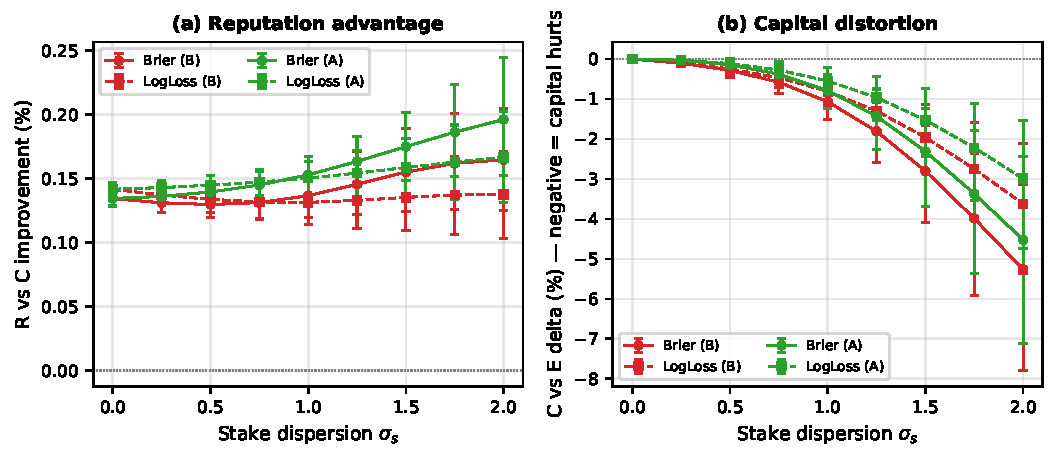
\includegraphics[width=\textwidth]{fig_inequality_sensitivity.pdf}
    \caption{Effect of stake dispersion ($\sigma_s$) on aggregation quality. \textbf{(a)}~Reputation advantage (R~vs~C improvement) grows with inequality across both regimes and both scoring rules. \textbf{(b)}~Capital distortion (C~vs~E delta) worsens monotonically with inequality; negative values indicate capital-weighting degrades the forecast. The reputation correction in~(a) grows far more slowly than the distortion in~(b), illustrating the architectural limitation of multiplicative weighting. Error bars: 95\% bootstrap CI ($n = 20$ seeds).}
    \label{fig:inequality}
\end{figure*}

The distortion is monotonically increasing in magnitude: at $\sigma_s = 2.0$, the capital-weighted forecast is $5.27\%$ worse than equal-weighting. Each increment of $\sigma_s$ worsens the distortion, with no plateau or reversal. In Regime~A (uncorrelated), the same pattern holds but with smaller magnitudes---C-vs-E reaches $-4.52\%$ at $\sigma_s = 2.0$---because random (rather than systematic) overweighting of noisy agents is less damaging than systematic overweighting.

\smallskip\noindent\textbf{Finding 10: The reputation correction grows with wealth inequality, but far more slowly than the distortion it corrects---because multiplicative reputation cannot override the stake floor of noisy whales.} Table~\ref{tab:recovery} reports the R-vs-C Brier improvement alongside the capital distortion for Regime~B, together with the fraction of distortion recovered.

\begin{table}[t]
\centering
\caption{Reputation Recovery vs.\ Capital Distortion (Regime~B, Brier)}
\label{tab:recovery}
\begin{tabular}{@{}cccc@{}}
\toprule
$\sigma_s$ & \textbf{C vs E (\%)} & \textbf{R vs C (\%)} & \textbf{Recovery} \\
\midrule
0.00 & $0.000$   & $+0.134$ & --- \\
0.25 & $-0.103$  & $+0.131$ & ${>}100\%$ \\
0.50 & $-0.281$  & $+0.130$ & $46\%$ \\
0.75 & $-0.580$  & $+0.131$ & $23\%$ \\
1.00 & $-1.068$  & $+0.137$ & $13\%$ \\
1.25 & $-1.807$  & $+0.146$ & $8\%$ \\
1.50 & $-2.802$  & $+0.155$ & $6\%$ \\
1.75 & $-3.988$  & $+0.162$ & $4\%$ \\
2.00 & $-5.265$  & $+0.165$ & $3\%$ \\
\bottomrule
\end{tabular}
\end{table}

The R-vs-C improvement grows from $+0.134\%$ to $+0.165\%$---a 23\% increase across the full range of~$\sigma_s$. But the capital distortion grows from $0\%$ to $-5.27\%$---a divergence of over two orders of magnitude. The recovery ratio collapses because the distortion is driven by noisy whales whose stake grows with~$\sigma_s$, while the reputation correction---a small multiplicative adjustment on those same stakes---scales proportionally to the stake, not to the damage the stake causes. As whales grow larger, reputation can only shave a few percent off their influence; it cannot shrink them down to the level their accuracy warrants. At moderate inequality ($\sigma_s = 0.50$, Gini~$\approx 0.25$), reputation recovers nearly half the capital distortion. But at extreme inequality ($\sigma_s = 2.0$, Gini~$\approx 0.73$), it recovers only 3\%. The same pattern holds in Regime~A, where R-vs-C grows from $+0.134\%$ to $+0.196\%$.

\smallskip\noindent\textbf{Finding 11: The multiplicative form is the binding constraint.} The fundamental limitation is architectural. Under multiplicative reputation-weighting, influence is $w_i = r_i \cdot s_i$: reputation \emph{scales} the stake but cannot \emph{replace} it. This means that a noisy whale's influence has a floor determined by their stake, regardless of how poor their track record becomes. Consider the numbers from this simulation: the reputation mechanism achieves a separation ratio of $1.107\times$---good agents converge to mean reputation ${\sim}0.89$, bad agents to ${\sim}0.80$ (both below the initial value of 1.0, since the exponential credit $\exp(-k(p-Y)^2)$ is almost always below~1 for $k=5$). Now consider two agents under extreme inequality ($\sigma_s = 2.0$):
\begin{itemize}
    \item A \emph{consistently accurate} small agent: reputation 0.89, stake 0.5 $\rightarrow$ effective weight \textbf{0.45}
    \item A \emph{consistently noisy} whale: reputation 0.80, stake 20 $\rightarrow$ effective weight \textbf{16.0}
\end{itemize}
The noisy whale exerts $36\times$ more influence on the aggregate forecast than the accurate small agent, despite the mechanism correctly identifying the whale as a poor forecaster. The reputation correction reduces the whale's weight by only 10\% (from~20 to~16)---a marginal adjustment relative to the underlying $40\times$ stake asymmetry. No matter how many rounds the small agent forecasts accurately, their effective weight cannot grow beyond $r_i \cdot s_i$, which is capped by their modest stake. The mechanism correctly identifies who is good and who is bad; the problem is that multiplicative reputation lacks the authority to act on that information when stakes are sufficiently concentrated. This motivates alternative weighting architectures---such as reputation-only weighting ($w_i = r_i$) or log-scaled stakes ($w_i = r_i \cdot \log(1 + s_i)$)---explored in Section~\ref{sec:discussion}.

\smallskip\noindent\textbf{Finding 12: Reputation separation is invariant to stake dispersion.} Across all 9 values of $\sigma_s$ and both regimes, the reputation separation ratio is exactly $1.107\times$ (to machine precision). The mechanism's ability to distinguish good from bad agents is determined entirely by the signal structure ($\sigma_{\text{good}}$, $\sigma_{\text{bad}}$, $J$) and the learning parameters ($\lambda$, $k$), not by the wealth distribution. (The slight difference from the $1.105\times$ reported in Section~\ref{sec:results-main} reflects different seed counts across campaigns---30 seeds in~\ref{sec:results-main} vs.\ 20 seeds here---not a change in mechanism behavior.) This invariance is a desirable property: the reputation signal is not contaminated by wealth structure. It also confirms that the limited recovery in Table~\ref{tab:recovery} is not due to a failure of reputation learning---the mechanism learns just as well under extreme inequality. The bottleneck is the weighting architecture, not the learning rule.

\subsection{Summary of Findings}
\label{sec:results-summary}

Table~\ref{tab:findings} consolidates the twelve findings. The results establish two complementary conclusions: (1)~capital-weighted aggregation degrades forecast quality under wealth--skill misalignment, and the degradation scales with wealth inequality; (2)~multiplicative reputation-weighting provides a consistent, safe, but modest correction---the mechanism reliably learns who is accurate and who is not, but the multiplicative architecture limits its ability to act on that knowledge, because a noisy whale's influence is floored by their stake regardless of their track record. Together, these findings motivate the search for weighting architectures that decouple influence from raw capital, giving reputation more authority relative to stake.

\begin{table*}[t]
\centering
\caption{Summary of Findings}
\label{tab:findings}
\begin{tabular}{@{}cp{9.5cm}p{5.5cm}@{}}
\toprule
\textbf{\#} & \textbf{Finding} & \textbf{Gap Addressed} \\
\midrule
1  & Reputation improves over capital in all 3 regimes ($p < 10^{-15}$); effect is modest ($+0.13$--$0.17\%$) & Performance-weighting beats capital-weighting [\ref{sec:related-aggregation}] \\
2  & Capital-weighting degrades forecasts in Regimes A ($-0.83\%$) and B ($-1.21\%$) & Capital = wealth-weighting, not info-weighting [\ref{sec:related-markets}] \\
3  & Reputation never underperforms capital, but correction is partial & Safety of adoption [\ref{sec:related-aggregation}] \\
4  & Reputation separation invariant to wealth structure ($1.105\times$) & --- \\
5  & Reputation advantage scales with noise gap & Effect under varying skill heterogeneity [\ref{sec:related-aggregation}] \\
6  & Reputation advantage scales with tail heaviness ($\alpha$) & Performance under heavy tails untested [\ref{sec:related-tails}] \\
7  & No parameter configuration where reputation hurts & Robustness [\ref{sec:related-gaps}] \\
8  & $\sigma_s = 0$: capital $\equiv$ equal (sanity check) & --- \\
9  & Capital distortion scales with inequality ($0\% \to -5.27\%$) & No test of wealth inequality variation [\ref{sec:related-markets}] \\
10 & Reputation advantage grows with inequality, but far slower than distortion (recovery: $46\% \to 3\%$) & No test of wealth inequality variation [\ref{sec:related-markets}] \\
11 & Multiplicative weighting is the binding constraint; ${\sim}10\%$ rep.\ differential cannot overcome $40\times$ stake differential & --- (central limitation) \\
12 & Reputation separation invariant to $\sigma_s$; learning works, architecture is the bottleneck & --- \\
\bottomrule
\end{tabular}
\end{table*}

% ============================================================
\section{Discussion}
\label{sec:discussion}
% ============================================================

\subsection{Interpretation of Effect Sizes}
\label{sec:discussion-effect}

The reputation-weighted improvement over capital-weighted aggregation is modest in absolute terms: $+0.13\%$ to $+0.20\%$ in Brier score across all tested configurations. This demands an honest assessment of what the effect means---and does not mean---in practice.

The effect is \emph{statistically} unambiguous. Across all six main results (3 regimes $\times$ 2 metrics), 95\% confidence intervals are entirely above zero, with $p$-values below $10^{-15}$. Across the 36-cell parameter sweep, the point estimate is non-negative in every cell, and 34 of 36 reach significance at $p < 0.05$. The mechanism never hurts. This consistency is the strongest form of the result: reputation-weighting is a safe, monotonic improvement over capital-weighting under every tested condition.

The effect is \emph{practically} small under default parameters, but it scales with the parameters that matter most. The improvement grows with the noise gap (from $+0.01\%$ at $\Delta\sigma = 0.5$ to $+0.50\%$ at $\Delta\sigma = 1.5$), with tail heaviness (larger $\alpha$ yields cleaner reputation learning), and with wealth inequality (from $+0.134\%$ at $\sigma_s = 0$ to $+0.196\%$ at $\sigma_s = 2.0$ in Regime~A). In the environments where capital-weighting causes the most damage---high inequality, anti-correlated wealth and skill, heavy tails---the reputation correction is largest.

Heavy-tailed outcomes amplify the consequences of miscalibration. In a thin-tailed setting where most items have similar outcomes, overweighting a noisy agent distorts the forecast only slightly---the forecast was close to the base rate regardless. In a heavy-tailed setting, rare extreme winners carry disproportionate value. A miscalibrated probability on a breakout event means misallocated attention, capital, and credit. The $+0.15\%$ Brier improvement we observe is an average across 5,000 rounds dominated by non-events (base rate $\approx 10\%$); the marginal improvement on the rounds that matter most---the tail events---may be substantially larger, though our experimental design does not isolate this. Future work could condition the analysis on tail events to quantify this hypothesis.

\subsection{Why Reputation Cannot Fully Compensate}
\label{sec:discussion-limits}

The inequality sensitivity sweep (Section~\ref{sec:results-inequality}) reveals the central architectural constraint of the mechanism tested in this paper. As wealth concentration increases, capital-weighted aggregation degrades sharply---from 0\% distortion at $\sigma_s = 0$ to $-5.27\%$ at $\sigma_s = 2.0$ in Regime~B. Reputation-weighted aggregation corrects for this, but the correction grows far more slowly than the distortion: the recovery ratio falls from 46\% at moderate inequality to just 3\% at extreme inequality (Table~\ref{tab:recovery}).

\begin{figure}[t]
    \centering
    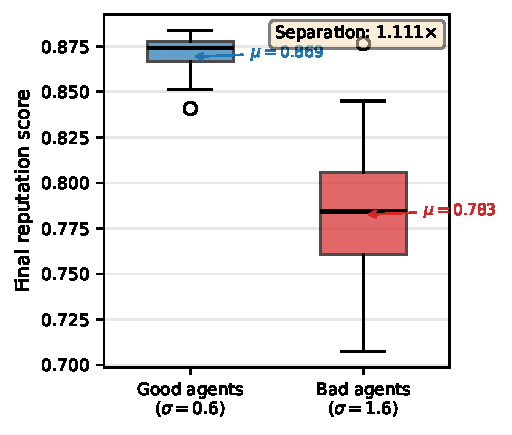
\includegraphics[width=\columnwidth]{fig_reputation_separation.pdf}
    \caption{Final reputation scores for good vs.\ bad agents after $J = 5{,}000$ rounds (Regime~B, seed~42). The mechanism achieves a $1.107\times$ separation ratio, correctly identifying agent quality---but the modest differential cannot override large stake asymmetries under multiplicative weighting.}
    \label{fig:rep-separation}
\end{figure}

The mechanism \emph{learns} correctly at all inequality levels. The reputation separation ratio is invariant to $\sigma_s$---the learning rule identifies agent quality from forecasting accuracy alone, uncontaminated by wealth structure (Finding~12). The bottleneck is not learning but \emph{authority}: under multiplicative weighting ($w_i = r_i \cdot s_i$), reputation can modulate a whale's influence by a small factor but cannot override it. A noisy whale with stake $20\times$ and reputation~0.80 still commands an effective weight of~16.0, dominating an accurate minnow with stake $0.5\times$ and reputation~0.89 (effective weight~0.45). The mechanism knows who is good---it simply cannot act on that knowledge proportionally.

This separation between learning and authority has a direct design implication. The reputation update rule (the EMA with exponential credit) performs well---it is fast enough to separate agents within hundreds of rounds and stable enough to resist single-round noise. The limitation is in the \emph{weighting architecture}, not the \emph{learning rule}. This means the appropriate next step is not to improve how reputation is learned, but to change how it is applied. The three candidate architectures identified in Section~\ref{sec:limitations}---multiplicative, reputation-only, and log-scaled---represent increasing degrees of authority transfer from capital to reputation. The calibration-vs-participation tradeoff across these architectures is the key open question for mechanism design.

\subsection{Implications for Market Design}
\label{sec:discussion-design}

In cultural markets, demonstrated early conviction already has revealed economic value. Fans trade proof of early discovery---screenshots of following an artist before their breakout, early playlist additions, timestamped listening history---as social currency, with observable secondary-market transactions for these artifacts. This behavior reveals latent demand for a system that converts conviction into verifiable taste: a record that is trustworthy, not forgeable, and that can compound over time as a forecaster demonstrates consistent accuracy.

The mechanism studied in this paper provides the infrastructure for exactly this. In a reputation-weighted prediction market, participants express cultural conviction as probabilistic forecasts---not as screenshots or social posts, but as quantified beliefs with economic stakes. Outcomes resolve (a track breaks out or it does not), and the forecasting record accumulates into a reputation score. The reputation is the verifiable taste: not a single early call, but a demonstrated pattern of calibrated prediction across many events. Our results validate the core premise of this design: when influence scales with accuracy rather than capital alone, the aggregate forecast improves. The improvement is consistent (Finding~1), safe---it never degrades performance even when capital already correlates with skill (Finding~3)---and robust across parameter configurations (Finding~7).

The composability of reputation is what distinguishes this from informal social proof. A screenshot proves presence but not prediction; it captures one moment but does not accumulate into a track record; and it cannot feed downstream decision systems. A reputation score derived from a prediction market is all of these: it is earned through repeated, verifiable accuracy; it compounds over time; and it is composable---it can weight future market influence, serve as an input to underwriting pipelines (as discussed in Section~\ref{sec:limitations} for cultural IP acquisition), or function as a portable credential of demonstrated taste. In this framing, the prediction market is not merely an information aggregation tool---it is a \emph{taste verification system} that produces a new kind of asset: verifiable, composable, accuracy-derived reputation. We refer to this design principle as \emph{Scenius}, after Brian Eno's concept of the communal form of genius that emerges from creative scenes~\cite{eno2009}. The term captures the mechanism's core function: surfacing the distributed intelligence of a cultural community by weighting demonstrated taste over capital concentration.

This reframing also clarifies why the capital-weighting problem documented in this paper is not merely a technical curiosity. In cultural markets, the participants with the best forward-looking information---early fans, tastemaker curators, niche community members---are systematically not the wealthiest market participants. This is Regime~B (anti-correlated) as a structural feature, not an edge case. Capital-weighted aggregation in this setting does not just introduce noise---it systematically underweights the most informed voices. Our finding that capital-weighting degrades forecast quality by up to $5.27\%$ in the anti-correlated regime (Finding~9), while reputation-weighting consistently corrects in the right direction (Findings~1, 10), provides the empirical basis for designing markets that take this structural feature seriously. Under reputation-weighting, tastemakers gain influence---and thus the ability to profit---in proportion to their demonstrated taste, instead of being underweighted and effectively extracted by capital-weighted aggregation.

The broader principle extends beyond cultural markets. Any domain where payoffs are heavy-tailed, private information is heterogeneous, and wealth does not proxy for expertise faces the same capital-weighting pathology. The specific degree of improvement will depend on domain-specific parameters---the noise gap, the tail heaviness, the degree of wealth--skill misalignment---but the direction of the result is structural: accuracy-weighted influence improves on capital-weighted influence when capital is a poor proxy for information quality.

% ============================================================
\section{Limitations and Future Work}
\label{sec:limitations}
% ============================================================

\subsection{Limitations}
\label{sec:limitations-limits}

The results in this paper should be interpreted in light of several modeling simplifications.

\textbf{One-shot aggregation, not a full market.} The central limitation is that our experiment uses a one-shot weighted average of beliefs rather than a full prediction market. Each round, agents report probabilities and we aggregate them once under three weighting rules. There is no order book, no sequential trading, no LMSR cost function, no liquidity pool, and no price impact. Real prediction markets produce prices through a dynamic process in which traders condition on observed prices, time their entries, and face liquidity constraints. We test whether reputation-weighting improves \emph{this kind} of static aggregation under heavy tails and heterogeneous skill. Whether the same advantage holds in a dynamic market---where strategic timing, information cascades, and market-maker mechanics introduce additional structure---is an open question that requires a fundamentally different simulation architecture.

\textbf{Multiplicative weighting architecture.} As documented in Finding~11, reputation is applied multiplicatively on top of stakes ($w_i = r_i \cdot s_i$). This architectural choice bounds the corrective power of reputation: a noisy whale's influence can be modulated but not overridden, because the stake sets a floor on effective weight. The mechanism correctly identifies agent quality (reputation separation is invariant across all tested conditions) but lacks the authority to act fully on that information under extreme wealth concentration. This is a limitation of the specific weighting architecture tested, not of reputation-weighting in general---alternative architectures may perform differently.

\textbf{Static stakes.} Each agent's stake is drawn once and held constant throughout the simulation. Real market participants dynamically allocate capital across rounds---sizing positions larger when confident, reducing exposure after losses, or exiting entirely. Dynamic capital allocation introduces feedback between performance and influence that our model does not capture. In particular, a reputation mechanism in a dynamic-stakes setting might interact with agents' capital allocation strategies in ways that amplify or dampen the effects documented here.

\textbf{Honest reporting.} All agents report their beliefs truthfully. The exponential credit function used for reputation updates is closely related to the Brier score and therefore incentive-compatible under truthful reporting. However, we do not model strategic behavior: agents do not manipulate their forecasts to game the reputation system, do not collude, and do not engage in Sybil attacks (splitting capital across multiple identities to diversify reputation risk). The robustness of the reputation mechanism to strategic manipulation is untested.

\textbf{Binary outcomes.} The simulation uses binary breakout events ($Y_j \in \{0, 1\}$). Real cultural markets produce continuous outcomes---a song may accumulate 500 streams or 50 million. Extending the model to continuous outcomes would require replacing the Bernoulli realization with a continuous payoff distribution and adapting both the scoring rules and the reputation update accordingly. Whether reputation-weighting retains its advantage under continuous outcomes is unknown.

\textbf{Modest effect sizes.} The reputation correction ranges from $+0.13\%$ to $+0.20\%$ in Brier score across all tested configurations. While statistically significant ($p < 10^{-7}$ in all main results), the practical magnitude is small. The significance is driven by consistency across seeds and rounds, not by large per-round improvements. Whether this modest effect translates to economically meaningful differences in a deployed market---where transaction costs, slippage, and participation incentives also matter---is an empirical question beyond the scope of this simulation.

\subsection{Future Work}
\label{sec:limitations-future}

\textbf{Alternative weighting architectures.} The most direct extension is to compare the multiplicative architecture against alternatives that give reputation more authority relative to stake. We propose three candidates:
\begin{enumerate}
    \item \emph{Multiplicative} (this paper): $w_i = r_i \cdot s_i$. Stake sets the floor; reputation is a marginal adjustment.
    \item \emph{Reputation-only}: $w_i = r_i$. Influence is determined entirely by track record, decoupled from capital. This maximizes reputation's corrective power but eliminates the skin-in-the-game incentive that capital provides.
    \item \emph{Reputation $\times$ log-scaled stake}: $w_i = r_i \cdot \log(1 + s_i)$. Stake has diminishing returns, so doubling capital does not double influence. Reputation has proportionally more bite without fully abandoning the participation incentive of staking. A variant, $w_i = \log(1 + r_i \cdot s_i)$, compresses the joint weight instead.
\end{enumerate}
The key tradeoff is between \emph{calibration} (how well the aggregate forecast reflects true probabilities) and \emph{participation} (whether agents have sufficient incentive to stake capital and reveal information). Multiplicative weighting maximizes participation incentives but limits calibration correction. Reputation-only weighting maximizes calibration correction but may reduce participation. Log-scaled weighting is a compromise. Future work should evaluate all three on both dimensions, ideally under strategic agents who respond to the incentive structure.

\textbf{Full LMSR and order-book markets.} Extending from one-shot aggregation to a sequential market with an LMSR cost function or a continuous double auction would test whether the reputation advantage survives when agents can condition on prices, trade strategically, and face liquidity constraints. The LMSR framework is particularly natural because the cost function parameter~$b$ controls liquidity depth, and reputation could be integrated either as a modifier on trade size (analogous to our multiplicative approach) or as a constraint on maximum position (analogous to log-scaling). This extension requires modeling agent trading strategies, which substantially increases simulation complexity.

\textbf{Strategic behavior and manipulation.} Agents in a deployed reputation system have incentives to game the mechanism: reporting conservatively to accumulate reputation before placing large bets, creating multiple identities to hedge reputation risk, or colluding to inflate each other's reputations. The EMA-based reputation update ($\lambda = 0.05$) provides some robustness through slow adaptation, but a systematic analysis of attack vectors and countermeasures---drawing on the mechanism design literature---is needed before deployment.

\textbf{Dynamic capital allocation.} Allowing agents to vary their stake across rounds based on confidence, past performance, or observed market conditions would introduce realistic feedback between reputation, capital, and forecasting behavior. This is particularly important for assessing whether reputation-weighting changes the \emph{composition} of market participation: does it attract more skilled forecasters (who benefit from the mechanism) or discourage large capital providers (whose influence is diluted)?

\textbf{Application to cultural IP underwriting.} In cultural IP acquisition---labels signing artists, studios greenlighting films, platforms licensing content---decision-makers face underwriting problems with heavily skewed payoffs: most bets fail, a few generate outsized returns. A concrete example is the emerging class of balance-sheet allocators that acquire music royalty streams and catalog rights. Duetti, a music fintech that has raised over \$435M to acquire catalogs from independent artists~\cite{duetti2025}, underwrites these acquisitions using backward-looking consumption data: streaming decay curves, listener counts, and historical volume~\cite{cohencircle2024}. This actuarial approach works well for established catalogs with years of data, but is inherently limited for early-career artists where historical signals are sparse yet crowd conviction about breakout potential may already exist. Our results suggest that forward-looking, reputation-weighted conviction markets can complement these data-driven underwriting pipelines: calibrated breakout probabilities derived from forecasters with demonstrated accuracy provide a signal that is unavailable from consumption data alone, particularly for artists at the inflection point between obscurity and breakout. The finding that reputation-weighting improves calibration under heavy-tailed outcomes (Finding~1) and that the advantage is robust across wealth--skill regimes (Findings~1--3) is directly relevant to this use case, where the payoff distribution is heavily skewed and the forecasters with the best information (tastemakers, early fans, A\&R scouts) may not be the wealthiest market participants. Validating this in a deployed market---where reputation-weighted probabilities feed real acquisition decisions and outcomes are observed---would close the loop between mechanism design and economic value.

\textbf{Generality beyond cultural markets.} The simulation uses Pareto-distributed outcomes and heterogeneous private signals---structural features shared by many domains beyond cultural breakout prediction. Venture capital forecasting (which startups will succeed), credit default risk (which borrowers will fail), token launch outcomes, and pharmaceutical trial prediction all exhibit heavy-tailed payoffs and uneven private information. Extending the empirical test to calibrated parameters from these domains would establish the mechanism's generality and identify domain-specific conditions under which reputation-weighting is most valuable.

\textbf{Continuous outcomes and multi-class prediction.} Replacing binary breakout with continuous payoffs (e.g., predicting streaming counts or revenue) or multi-class outcomes (e.g., ranking content into tiers) would broaden the mechanism's applicability. This requires extending the scoring and reputation update rules to continuous proper scoring rules (e.g., the CRPS) or multi-class generalizations of the Brier score.

% ============================================================
\section{Conclusion}
\label{sec:conclusion}
% ============================================================

Capital-weighted prediction markets embed the assumption that willingness to stake capital proxies for information quality. This paper tests that assumption under controlled variation in wealth inequality, wealth--skill correlation, and outcome tail heaviness---and finds it wanting. When wealth does not positively correlate with forecasting skill, capital-weighting degrades the aggregate forecast, and the degradation scales monotonically with wealth concentration---reaching $-5.27\%$ in Brier score under extreme inequality with anti-correlated wealth and skill.

Reputation-weighted aggregation provides a consistent corrective. By scaling each agent's influence by a learned reputation score derived from demonstrated forecasting accuracy, the mechanism improves calibration in every tested configuration: across all three wealth--skill regimes, all parameter sweep cells, and all inequality levels. The improvement is statistically significant ($p < 10^{-15}$ in main results), robust across tail heaviness and signal heterogeneity, and safe---there is no configuration in which it degrades performance.

The effect is modest under the multiplicative architecture tested here ($+0.13\%$ to $+0.20\%$ in Brier score), and this modesty is itself an important finding. The mechanism correctly identifies agent quality---reputation separation is invariant across all tested conditions---but the multiplicative form $w_i = r_i \cdot s_i$ limits its authority to act on that knowledge. A ${\sim}10\%$ reputation differential cannot override a $40\times$ stake differential. The bottleneck is the weighting architecture, not the learning rule. This motivates a clear next step: evaluating alternative architectures---reputation-only weighting, log-scaled stakes, or other forms that give demonstrated accuracy greater authority relative to raw capital---to determine how much of the capital-weighting distortion can be recovered.

More broadly, this work provides empirical grounding for a design principle: in markets where payoffs are heavy-tailed and wealth is a poor proxy for expertise, influence should scale with demonstrated accuracy, not just capital. In cultural markets specifically, where early conviction about breakout potential is valuable but systematically held by participants who are not the wealthiest, reputation-weighted aggregation offers a path toward converting that conviction into verifiable, composable taste---and functionally, into an asset.

% ============================================================
% References
% ============================================================

\balance
\bibliographystyle{IEEEtran}
\bibliography{references}

\end{document}
